\subsubsection{tick}
    Enthält die Datenstruktur Tick und Funktionalität um die Datenstruktur zwischen Simulations- und RenderThread zu übergeben.

    \begin{figure}[htbp]
        \centering
        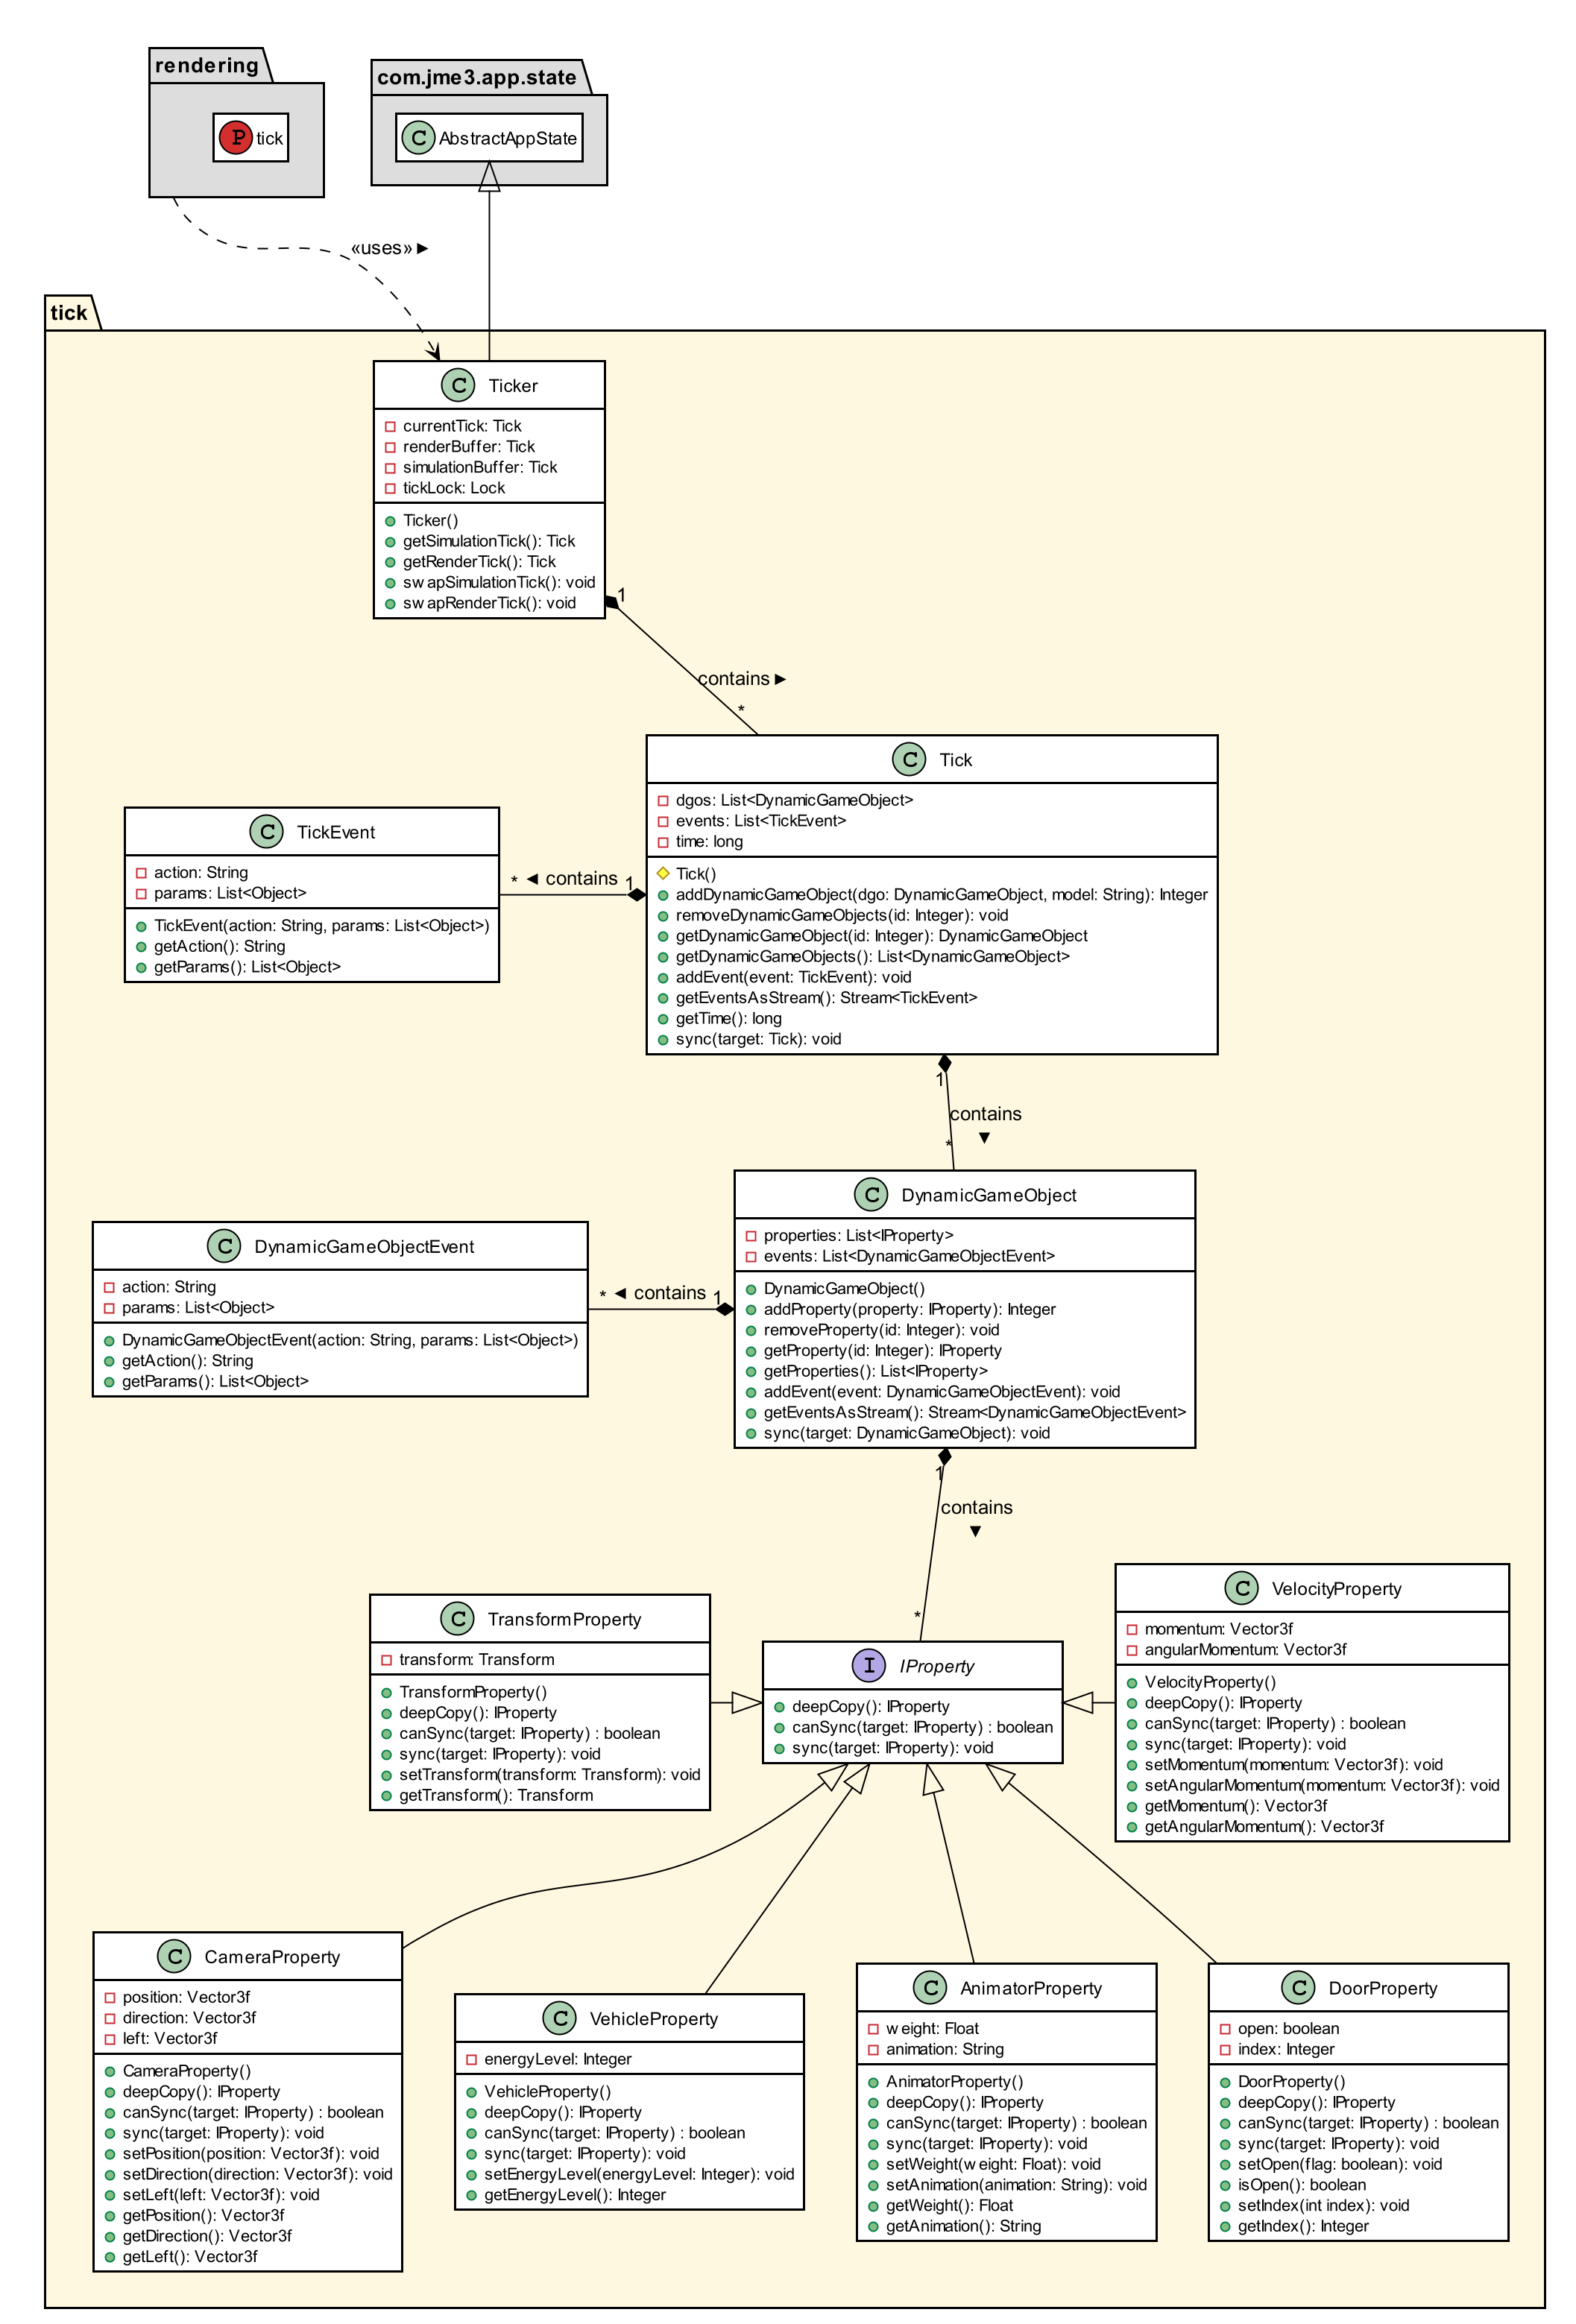
\includegraphics[width=0.72\linewidth]{Interface/tick.png}
        \caption{tick Klassen-Diagram}
    \end{figure}

    \paragraph{\underline{Ticker}} \mbox{}\\
    \\
        AbstractAppState, welcher die Buffer für triple-buffering zwischen Simulations- und RenderThread hält und das triple-buffering kontrolliert.\par
        
        \textbf{Attribute}
        \begin{itemize}
            \item \textit{- Tick simulationBuffer}
                \begin{leftbar}[0.9\linewidth]
                    \textit{Tick} welcher vom SimulationsThread verwendet wird.
                \end{leftbar}
            \item \textit{- Tick renderBuffer}
                \begin{leftbar}[0.9\linewidth]
                    \textit{Tick} welcher vom RenderThread verwendet wird.
                \end{leftbar}
            \item \textit{- Tick currentTick}
                \begin{leftbar}[0.9\linewidth]
                    \textit{Tick} welcher den aktuellsten stand der Szene hält.
                \end{leftbar}
            \item \textit{- Lock tickLock}
                \begin{leftbar}[0.9\linewidth]
                    Wird verwendet um die Zugriffe auf die Methoden \textit{Ticker.swapSimulationBuffer} und \textit{Ticker.swapRenderBuffer}
                    zu synchronisieren.
                \end{leftbar}
        \end{itemize}

        \textbf{Methoden}
        \begin{itemize}
            \item \textit{+ Ticker()}
                \begin{leftbar}[0.9\linewidth]
                    Erstellt einen neuen \textit{Ticker} und initialisiert simulationBuffer, renderBuffer und currentTick als neuen \textit{Tick} und tickLock
                    als neues ReentrantLock.
                \end{leftbar}
            \item \textit{+ getSimulatioTick(): Tick}
                \begin{leftbar}[0.9\linewidth]
                    \textbf{@return} den \textit{Tick}, welcher vom SimulationsThread verwendet wird.
                \end{leftbar}
            \item \textit{+ getRenderTick(): Tick}
                \begin{leftbar}[0.9\linewidth]
                    \textbf{@return} den \textit{Tick}, welcher vom RenderThread verwendet wird.
                \end{leftbar}
            \item \textit{+ swapSimulationTick(): void}
                \begin{leftbar}[0.9\linewidth]
                    Überträgt den stand von simulationBuffer in currentTick.
                \end{leftbar}
            \item \textit{+ swapRenderTick(): void}
                \begin{leftbar}[0.9\linewidth]
                    Überträgt den stand von currentTick in renderBuffer.
                \end{leftbar}
        \end{itemize}

    \pagebreak
    \paragraph{\underline{Tick}} \mbox{}\\
    \\
        Enthält alle \textit{DynamicGameObject}s und \textit{TickEvent}s.\par
        
        \textbf{Attribute}
        \begin{itemize}
            \item \textit{- List<DynamicGameObject> dgos}
                \begin{leftbar}[0.9\linewidth]
                    Enthält alle momentan aktiven \textit{DynamicGameObject}s.
                \end{leftbar}
            \item \textit{- List<TickEvent> events}
                \begin{leftbar}[0.9\linewidth]
                    Enthält alle \textit{TickEvent}s.
                \end{leftbar}
            \item \textit{- long time}
                \begin{leftbar}[0.9\linewidth]
                    Wie viele Millisekunden zwischen den letzten 2 \textit{Tick.sync()} Aufrufen lagen.
                \end{leftbar}
        \end{itemize}

        \textbf{Methoden}
        \begin{itemize}
            \item \textit{\# Tick()}
                \begin{leftbar}[0.9\linewidth]
                    Erstellt einen neuen \textit{Tick} und initialisiert dgos und events als leere List und time als 0.
                \end{leftbar}
            \item \textit{+ addDynamicGameObject(DynamicGameObject dgo, String model): int}
                \begin{leftbar}[0.9\linewidth]
                    Fügt ein neues \textit{DynamicGameObject} hinzu.\\
                    \textbf{@param dgo} das \textit{DynamicGameObject}, welches hinzugefügt werden soll.\\
                    \textbf{@param model} das Asset, welches dieses \textit{DynamicGameObject} im Scenegraph repräsentiert.\\
                    \textbf{@return} den Index, an dem das \textit{DynamicGameObject} eingefügt wurde.
                \end{leftbar}
            \item \textit{+ removeDynamicGameObject(int index): void}
                \begin{leftbar}[0.9\linewidth]
                    Entfernt das \textit{DynamicGameObject} am gegebenen Index.\\
                    \textbf{@param index} der Index des \textit{DynamicGameObject}s, welches entfernt werden soll.
                \end{leftbar}
            \item \textit{+ getDynamicGameObject(int index): DynamicGameObject}
                \begin{leftbar}[0.9\linewidth]
                    Gibt das \textit{DynamicGameObject} am gegebenen Index zurück.\\
                    \textbf{@param index} der Index des \textit{DynamicGameObject}s.\\
                    \textbf{@return } das \textit{DynamicGameObject} am gegebenen Index.
                \end{leftbar}
            \item \textit{+ getDynamicGameObjects(): List<DynamicGameObject>}
                \begin{leftbar}[0.9\linewidth]
                    Gibt alle \textit{DynamicGameObject}s als List zurück.\\
                    \textbf{@return } eine List, welche alle \textit{DynamicGameObject}s enthält.
                \end{leftbar}
            \item \textit{+ addEvent(TickEvent event): void}
                \begin{leftbar}[0.9\linewidth]
                    Fügt ein neues \textit{TickEvent} hinzu.\\
                    \textbf{@param event} das \textit{TickEvent}
                \end{leftbar}
            
            \pagebreak
            \item \textit{+ getEventsAsStream(): Stream<TickEvent>}
                \begin{leftbar}[0.9\linewidth]
                    Erstellt einen Stream, welcher alle \textit{TickEvent}s, die momentan in diesem \textit{Tick} enthalten sind
                    und entfernt danach alle \textit{TickEvent}s aus diesem \textit{Tick}.\\
                    \textbf{@return} der Stream, welcher alle \textit{TickEvent}s enthält.
                \end{leftbar}
            \item \textit{+ getTime(): long}
                \begin{leftbar}[0.9\linewidth]
                    \textbf{@return} Wie viele Millisekunden zwischen den letzten 2 Aufrufen von \textit{Tick.sync()} liegen.
                \end{leftbar}
            \item \textit{+ sync(Tick target): void}
                \begin{leftbar}[0.9\linewidth]
                    Synchronisiert diesen \textit{Tick} mit dem gegebenen in 2 Schritten:\\
                    1. Synchronisiert alle \textit{DynamicGameObject}s über die Methode \textit{DynamicGameObject.sync()}, neue \textit{DynamicGameObject}s
                    werden ggf. erstellt.\\
                    2. Hängt alle \textit{TickEvent}s aus target hinten an events an.\\
                    \textbf{@param target} der \textit{Tick} mit dem synchronisiert werden soll.
                \end{leftbar}
        \end{itemize}

    \paragraph{\underline{TickEvent}} \mbox{}\\
    \\
        Repräsentiert ein Event, welches auf der Datenstruktur \textit{Tick} auftritt.\par

        \textbf{Attribute}
        \begin{itemize}
            \item \textit{- String action}
                \begin{leftbar}[0.9\linewidth]
                    Nennt die Aktion, für welche dieses \textit{TickEvent} erstellt wurde.
                \end{leftbar}
            \item \textit{- List<Object> params}
                \begin{leftbar}[0.9\linewidth]
                    Enthält alle Parameter, welche für die Verarbeitung dieses \textit{TickEvent}s eine Rolle spielen.
                \end{leftbar}
        \end{itemize}

        \textbf{Methoden}
        \begin{itemize}
            \item \textit{+ TickEvent(String action, List<Object> params)}
                \begin{leftbar}[0.9\linewidth]
                    Erstellt ein neues \textit{TickEvent} und speichert die Parameter ab.\\
                    \textbf{@param action} die Aktion, für welche dieses \textit{TickEvent} erstellt wurde.\\
                    \textbf{@param params} alle Parameter, welche für die Verarbeitung dieses \textit{TickEvent}s eine Rolle spielen.
                \end{leftbar}
            \item \textit{+ getAction(): String}
                \begin{leftbar}[0.9\linewidth]
                    \textbf{@return} die Aktion, für welche dieses \textit{TickEvent} erstellt wurde.
                \end{leftbar}
            \item \textit{+ getParams(): List<Object>}
                \begin{leftbar}[0.9\linewidth]
                    \textbf{@return} alle Parameter, welche für die Verarbeitung dieses \textit{TickEvent}s eine Rolle spielen.
                \end{leftbar}
        \end{itemize}

        \paragraph{\underline{DynamicGameObject}} \mbox{}\\
        \\
            Repräsentiert ein dynamisches Objekt im Spiel.\par

            \textbf{Attribute}
            \begin{itemize}
                \item \textit{- List<IProperty> properties}
                    \begin{leftbar}[0.9\linewidth]
                        Enthält alle \textit{IProperty}s die dieses \textit{DynamicGameObject} definieren.
                    \end{leftbar}
                \item \textit{- List<DynamicGameObjectEvent> events}
                    \begin{leftbar}[0.9\linewidth]
                        Enthält alle \textit{DynamicGameObjectEvent}s die dieses \textit{DynamicGameObject} momentan enthält.
                    \end{leftbar}
            \end{itemize}

            \textbf{Methoden}
            \begin{itemize}
                \item \textit{+ DynamicGameObject()}
                    \begin{leftbar}[0.9\linewidth]
                        Erstellt ein neues \textit{DynamicGameObject} und initialisiert properties und events als leere List.
                    \end{leftbar}
                \item \textit{+ addProperty(IProperty property): int}
                    \begin{leftbar}[0.9\linewidth]
                        Fügt dem \textit{DynamicGameObject} eine neue \textit{IProperty} hinzu.\\
                        \textbf{@param property} die \textit{IProperty} welche hinzugefügt werden soll.\\
                        \textbf{@return} den Index der hinzugefügten \textit{IProperty}.
                    \end{leftbar}

                \item \textit{+ removeProperty(int id): void}
                    \begin{leftbar}[0.9\linewidth]
                        Entfernt eine \textit{IProperty} von diesem \textit{DynamicGameObject}.\\
                        \textbf{@param id} der Index der \textit{IProperty}, die entfernt werden soll.
                    \end{leftbar}
                \item \textit{+ getProperty(int id): IProperty}
                    \begin{leftbar}[0.9\linewidth]
                        \textbf{@return} die \textit{IProperty} mit dem gegebenen Index.
                    \end{leftbar}
                \item \textit{+ getProperties(): List<IProperty>}
                    \begin{leftbar}[0.9\linewidth]
                        \textbf{@return} eine List, welche alle \textit{IProperty}s dieses \textit{DynamicGameObject} enthält.
                    \end{leftbar}
                \item \textit{+ addEvent(DynamicGameObjectEvent event): void}
                    \begin{leftbar}[0.9\linewidth]
                        Fügt ein neues \textit{DynamicGameObjectEvent} diesem \textit{DynamicGameObject} hinzu.\\
                        \textbf{@param event} das \textit{DynamicGameObjectEvent}, das hinzugefügt werden soll.
                    \end{leftbar}
                \item \textit{+ getEventsAsStream(): Stream<DynamicGameObjectEvent>}
                    \begin{leftbar}[0.9\linewidth]
                        Entfernt alle \textit{DynamicGameObjectEvent}s aus diesem \textit{DynamicGameObject} und gibt sie in einem Stream zurück.\\
                        \textbf{@return} alle \textit{DynamicGameObjectEvent}s in einem Stream.
                    \end{leftbar}
                
                \pagebreak
                \item \textit{+ sync(DynamicGameObject target): void}
                    \begin{leftbar}[0.9\linewidth]
                        Synchronisiert dieses \textit{DynamicGameObject} mit dem gegebenen in 2 Schritten:\\
                        1. Synchronisiert alle \textit{IProperty}s miteinander, neue \textit{IProperty}s werden ggf. kopiert.\\
                        2. Hängt alle \textit{DynamicGameObjectEvent} hinten in die liste von \textit{DynamicGameObjectEvent}s.\\
                        \textbf{@param target} das \textit{DynamicGameObject} mit dem synchronisiert werden soll.
                    \end{leftbar}
            \end{itemize}

        \paragraph{\underline{DynamicGameObjectEvent}} \mbox{}\\
        \\
            Repräsentiert ein Event, welches auf der Datenstruktur DynamicGameObject auftritt.\par

            \textbf{Attribute}
            \begin{itemize}
                \item \textit{- String action}
                    \begin{leftbar}[0.9\linewidth]
                        Nennt die Aktion, für die dieses \textit{DynamicGameObjectEvent} erstellt wurde.
                    \end{leftbar}
                \item \textit{- List<Object> params}
                    \begin{leftbar}[0.9\linewidth]
                        Enthält alle zur Verarbeitung dieses \textit{DynamicGameObjectEvent}s relevanten Parameter.
                    \end{leftbar}
            \end{itemize}

            \textbf{Methoden}
            \begin{itemize}
                \item \textit{+ DynamicGameObjectEvent(String action, List<Object> params)}
                    \begin{leftbar}[0.9\linewidth]
                        Erstellt ein neues \textit{DynamicGameObjectEvent} und speichert die Parameter ab.\\
                        \textbf{@param action} die Aktion, für die dieses \textit{DynamicGameObjectEvent} erstellt wurde.\\
                        \textbf{@param params} die Parameter, welche für die Verarbeitung dieses \textit{DynamicGameObjectEvent}s eine Rolle spielen.
                    \end{leftbar}
                \item \textit{+ getAction(): String}
                    \begin{leftbar}[0.9\linewidth]
                        \textbf{@return} die Aktion, für die dieses \textit{DynamicGameObjectEvent} erstellt wurde.
                    \end{leftbar}
                \item \textit{+ getParams(): List<Object>}
                    \begin{leftbar}[0.9\linewidth]
                        \textbf{@return} alle Parameter, die für die Verarbeitung dieses \textit{DynamicGameObjectEvent}s eine Rolle spielen.
                    \end{leftbar}
            \end{itemize}

        \pagebreak
        \paragraph{\underline{IProperty}} \mbox{}\\
        \\
            Definiert die mindest funktionalität, damit die \textit{IProperty} von einem \textit{DynamicGameObject} verwendet werden kann.\par

            \textbf{Methoden}
            \begin{itemize}
                \item \textit{+ deepCopy(): IProperty}
                    \begin{leftbar}[0.9\linewidth]
                        \textbf{@return} eine Deep-Copy von sich selbst.
                    \end{leftbar}
                \item \textit{+ canSync(IProperty target): boolean}
                    \begin{leftbar}[0.9\linewidth]
                        \textbf{@return} ob diese \textit{IProperty} mit der gegebenen \textit{IProperty} synchronisiert werden kann.
                    \end{leftbar}
                \item \textit{+ sync(IProperty target): void}
                    \begin{leftbar}[0.9\linewidth]
                        Macht diese \textit{IProperty} zu einer Deep-Copy der gegebenen \textit{IProperty}, falls \textit{IProperty.canSync(target)} true zurück gibt.
                    \end{leftbar}
            \end{itemize}

        \paragraph{\underline{TransformProperty}} \mbox{}\\
        \\
            Eine \textit{IProperty} die Position, Rotation und Skalierung enthält.\par

            \textbf{Attribute}
            \begin{itemize}
                \item \textit{- Transform transform}
                    \begin{leftbar}[0.9\linewidth]
                        Ein Transform, welcher Position, Rotation und Skalierung enthält.
                    \end{leftbar}
            \end{itemize}

            \textbf{Methoden}
            \begin{itemize}
                \item \textit{+ deepCopy(): IProperty}
                    \begin{leftbar}[0.9\linewidth]
                        Siehe \textit{IProperty.deepCopy()}.
                    \end{leftbar}
                \item \textit{+ canSync(IProperty target): boolean}
                    \begin{leftbar}[0.9\linewidth]
                        Siehe \textit{IProperty.canSync()}.
                    \end{leftbar}
                \item \textit{+ sync(IProperty target): void}
                    \begin{leftbar}[0.9\linewidth]
                        Siehe \textit{IProperty.sync()}.
                    \end{leftbar}
                \item \textit{+ setTransform(Transform transform): void}
                    \begin{leftbar}[0.9\linewidth]
                        Setzt Position, Rotation und Skalierung.\\
                        \textbf{@param transform} der Transform, welcher Position, Rotation und Skalierung enthält.
                    \end{leftbar}

                \pagebreak
                \item \textit{+ getTransform(): Transform}
                    \begin{leftbar}[0.9\linewidth]
                        \textbf{@return} Position, Rotation und Skalierung in einem Transform.
                    \end{leftbar}
            \end{itemize}
            
        \paragraph{\underline{VelocityProperty}} \mbox{}\\
        \\
            Eine \textit{IProperty} die die Geschwindigkeit enthält.\par

            \textbf{Attribute}
            \begin{itemize}
                \item \textit{- Vector3f momentum}
                    \begin{leftbar}[0.9\linewidth]
                        Die Geschwindigkeit als Vector3f.
                    \end{leftbar}
                \item \textit{- Vector3f angularMomentum}
                    \begin{leftbar}[0.9\linewidth]
                        Die Winkelgeschwindigkeit als Vector3f.
                    \end{leftbar}
            \end{itemize}

            \textbf{Methoden}
            \begin{itemize}
                \item \textit{+ deepCopy(): IProperty}
                    \begin{leftbar}[0.9\linewidth]
                        Siehe \textit{IProperty.deepCopy()}.
                    \end{leftbar}
                \item \textit{+ canSync(IProperty target): boolean}
                    \begin{leftbar}[0.9\linewidth]
                        Siehe \textit{IProperty.canSync()}.
                    \end{leftbar}
                \item \textit{+ sync(IProperty target): void}
                    \begin{leftbar}[0.9\linewidth]
                        Siehe \textit{IProperty.sync()}.
                    \end{leftbar}
                \item \textit{+ setMomentum(Vector3f momentum): void}
                    \begin{leftbar}[0.9\linewidth]
                        Setzt die Geschwindigkeit.\\
                        \textbf{@param momentum} die Geschwindigkeit.
                    \end{leftbar}
                \item \textit{+ getMomentum(): Vector3f}
                    \begin{leftbar}[0.9\linewidth]
                        \textbf{@return} die Geschwindigkeit.
                    \end{leftbar}
                \item \textit{+ setAngularMomentum(Vector3f angularMomentum): void}
                    \begin{leftbar}[0.9\linewidth]
                        Setzt die Winkelgeschwindigkeit.\\
                        \textbf{@param angularMomentum} die Winkelgeschwindigkeit.
                    \end{leftbar}
                \item \textit{+ getAngularMomentum(): Vector3f}
                    \begin{leftbar}[0.9\linewidth]
                        \textbf{@return} die Winkelgeschwindigkeit.
                    \end{leftbar}
            \end{itemize}

        \paragraph{\underline{CameraProperty}} \mbox{}\\
        \\
            Eine \textit{IProperty} die Position, und Richtung der Camera, relativ zum DynamicGameObject welches diese IProperty enthält.\par

            \textbf{Attribute}
            \begin{itemize}
                \item \textit{- Vector3f position}
                    \begin{leftbar}[0.9\linewidth]
                        Die Position der Kamera.
                    \end{leftbar}
                \item \textit{- Vector3f direction}
                    \begin{leftbar}[0.9\linewidth]
                        Die Richtung der Kamera.
                    \end{leftbar}
                \item \textit{- Vector3f left}
                    \begin{leftbar}[0.9\linewidth]
                        Der Links-Vektor der Kamera.
                    \end{leftbar}
            \end{itemize}

            \textbf{Methoden}
            \begin{itemize}
                \item \textit{+ deepCopy(): IProperty}
                    \begin{leftbar}[0.9\linewidth]
                        Siehe \textit{IProperty.deepCopy()}.
                    \end{leftbar}
                \item \textit{+ canSync(IProperty target): boolean}
                    \begin{leftbar}[0.9\linewidth]
                        Siehe \textit{IProperty.canSync()}.
                    \end{leftbar}
                \item \textit{+ sync(IProperty target): void}
                    \begin{leftbar}[0.9\linewidth]
                        Siehe \textit{IProperty.sync()}.
                    \end{leftbar}
                \item \textit{+ setPosition(Vector3f position): void}
                    \begin{leftbar}[0.9\linewidth]
                        Setzt die Position der Kamera.\\
                        \textbf{@param position} die Position.
                    \end{leftbar}
                \item \textit{+ getPosition(): Vector3f}
                    \begin{leftbar}[0.9\linewidth]
                        \textbf{@return} die Position der Kamera.
                    \end{leftbar}
                \item \textit{+ setDirection(Vector3f direction): void}
                    \begin{leftbar}[0.9\linewidth]
                        Setzt die Richtung der Kamera.\\
                        \textbf{@param direcion} die Richtung.
                    \end{leftbar}
                \item \textit{+ getDirection(): Vector3f}
                    \begin{leftbar}[0.9\linewidth]
                        \textbf{@return} die Richtung der Kamera.
                    \end{leftbar}
                \item \textit{+ setLeft(Vector3f left): void}
                    \begin{leftbar}[0.9\linewidth]
                        Setzt den Links-Vektor der Kamera.\\
                        \textbf{@param left} derLinks-Vektor.
                    \end{leftbar}
                \item \textit{+ getLeft(): Vector3f}
                    \begin{leftbar}[0.9\linewidth]
                        \textbf{@return} den Links-Vektor der Kamera.
                    \end{leftbar}
            \end{itemize}

        \pagebreak
        \paragraph{\underline{VehicleProperty}} \mbox{}\\
        \\
            Eine \textit{IProperty} die das Energielevel des Fahrzeugs hält.\par

            \textbf{Attribute}
            \begin{itemize}
                \item \textit{- int energyLevel}
                    \begin{leftbar}[0.9\linewidth]
                        Der Energielevel des Fahrzeugs.
                    \end{leftbar}
            \end{itemize}

            \textbf{Methoden}
            \begin{itemize}
                \item \textit{+ deepCopy(): IProperty}
                    \begin{leftbar}[0.9\linewidth]
                        Siehe \textit{IProperty.deepCopy()}.
                    \end{leftbar}
                \item \textit{+ canSync(IProperty target): boolean}
                    \begin{leftbar}[0.9\linewidth]
                        Siehe \textit{IProperty.canSync()}.
                    \end{leftbar}
                \item \textit{+ sync(IProperty target): void}
                    \begin{leftbar}[0.9\linewidth]
                        Siehe \textit{IProperty.sync()}.
                    \end{leftbar}
                \item \textit{+ setEnergyLevel(int energyLevel): void}
                    \begin{leftbar}[0.9\linewidth]
                        Setzt den Energielevel dieses Fahrzeugs.\\
                        \textbf{@param energyLevel} der Energielevel.
                    \end{leftbar}
                \item \textit{+ getEnergyLevel(): int}
                    \begin{leftbar}[0.9\linewidth]
                        \textbf{@return} den Energielevel des Fahrzeugs.
                    \end{leftbar}
            \end{itemize}

        \paragraph{\underline{AnimatorProperty}} \mbox{}\\
        \\
            Eine \textit{IProperty} die eine momentan aktive Animation repräsentiert.\par

            \textbf{Attribute}
            \begin{itemize}
                \item \textit{- float weight}
                    \begin{leftbar}[0.9\linewidth]
                        Die Gewicht der Animation.
                    \end{leftbar}
                \item \textit{- String animation}
                    \begin{leftbar}[0.9\linewidth]
                        Der Name der Animation.
                    \end{leftbar}
            \end{itemize}

            \textbf{Methoden}
            \begin{itemize}
                \item \textit{+ deepCopy(): IProperty}
                    \begin{leftbar}[0.9\linewidth]
                        Siehe \textit{IProperty.deepCopy()}.
                    \end{leftbar}
                
                \pagebreak
                \item \textit{+ canSync(IProperty target): boolean}
                    \begin{leftbar}[0.9\linewidth]
                        Siehe \textit{IProperty.canSync()}.
                    \end{leftbar}
                \item \textit{+ sync(IProperty target): void}
                    \begin{leftbar}[0.9\linewidth]
                        Siehe \textit{IProperty.sync()}.
                    \end{leftbar}
                \item \textit{+ setWeight(float weight): void}
                    \begin{leftbar}[0.9\linewidth]
                        Setzt das Gewicht der Animation.\\
                        \textbf{@param weight} das Gewicht.
                    \end{leftbar}
                \item \textit{+ getWeight(): float}
                    \begin{leftbar}[0.9\linewidth]
                        \textbf{@return} das Gewicht der Animation.
                    \end{leftbar}
                \item \textit{+ setAnimation(float animation): void}
                    \begin{leftbar}[0.9\linewidth]
                        Setzt den Namen der Animation.\\
                        \textbf{@param animation} der Name der Animation.
                    \end{leftbar}
                \item \textit{+ getAnimation(): float}
                    \begin{leftbar}[0.9\linewidth]
                        \textbf{@return} den Namen der Animation.
                    \end{leftbar}
            \end{itemize}

        \paragraph{\underline{DoorProperty}} \mbox{}\\
        \\
            Eine \textit{IProperty} die den Status einer Tür enthält.\par

            \textbf{Attribute}
            \begin{itemize}
                \item \textit{- boolean open}
                    \begin{leftbar}[0.9\linewidth]
                        Ob die Tür offen oder geschlossen ist.
                    \end{leftbar}
                \item \textit{- int index}
                    \begin{leftbar}[0.9\linewidth]
                        Der Index der Tür.
                    \end{leftbar}
            \end{itemize}

            \textbf{Methoden}
            \begin{itemize}
                \item \textit{+ deepCopy(): IProperty}
                    \begin{leftbar}[0.9\linewidth]
                        Siehe \textit{IProperty.deepCopy()}.
                    \end{leftbar}
                \item \textit{+ canSync(IProperty target): boolean}
                    \begin{leftbar}[0.9\linewidth]
                        Siehe \textit{IProperty.canSync()}.
                    \end{leftbar}
                \item \textit{+ sync(IProperty target): void}
                    \begin{leftbar}[0.9\linewidth]
                        Siehe \textit{IProperty.sync()}.
                    \end{leftbar}
                
                \pagebreak
                \item \textit{+ setOpen(boolean flag): void}
                    \begin{leftbar}[0.9\linewidth]
                        Setzt ob die Tür offen oder geschlossen ist.\\
                        \textbf{@param flag} ob die Tür offen oder geschlossen ist.
                    \end{leftbar}
                \item \textit{+ isOpen(): boolean}
                    \begin{leftbar}[0.9\linewidth]
                        \textbf{@return} ob die Tür offen oder geschlossen ist.
                    \end{leftbar}
                \item \textit{+ setIndex(int index): void}
                    \begin{leftbar}[0.9\linewidth]
                        Setzt den Index der Tür.\\
                        \textbf{@param index} der Index der Tür.
                    \end{leftbar}
            \end{itemize}